\documentclass[1p]{elsarticle_modified}
%\bibliographystyle{elsarticle-num}

%\usepackage[colorlinks]{hyperref}
%\usepackage{abbrmath_seonhwa} %\Abb, \Ascr, \Acal ,\Abf, \Afrak
\usepackage{amsfonts}
\usepackage{amssymb}
\usepackage{amsmath}
\usepackage{amsthm}
\usepackage{scalefnt}
\usepackage{amsbsy}
\usepackage{kotex}
\usepackage{caption}
\usepackage{subfig}
\usepackage{color}
\usepackage{graphicx}
\usepackage{xcolor} %% white, black, red, green, blue, cyan, magenta, yellow
\usepackage{float}
\usepackage{setspace}
\usepackage{hyperref}

\usepackage{tikz}
\usetikzlibrary{arrows}

\usepackage{multirow}
\usepackage{array} % fixed length table
\usepackage{hhline}

%%%%%%%%%%%%%%%%%%%%%
\makeatletter
\renewcommand*\env@matrix[1][\arraystretch]{%
	\edef\arraystretch{#1}%
	\hskip -\arraycolsep
	\let\@ifnextchar\new@ifnextchar
	\array{*\c@MaxMatrixCols c}}
\makeatother %https://tex.stackexchange.com/questions/14071/how-can-i-increase-the-line-spacing-in-a-matrix
%%%%%%%%%%%%%%%

\usepackage[normalem]{ulem}

\newcommand{\msout}[1]{\ifmmode\text{\sout{\ensuremath{#1}}}\else\sout{#1}\fi}
%SOURCE: \msout is \stkout macro in https://tex.stackexchange.com/questions/20609/strikeout-in-math-mode

\newcommand{\cancel}[1]{
	\ifmmode
	{\color{red}\msout{#1}}
	\else
	{\color{red}\sout{#1}}
	\fi
}

\newcommand{\add}[1]{
	{\color{blue}\uwave{#1}}
}

\newcommand{\replace}[2]{
	\ifmmode
	{\color{red}\msout{#1}}{\color{blue}\uwave{#2}}
	\else
	{\color{red}\sout{#1}}{\color{blue}\uwave{#2}}
	\fi
}

\newcommand{\Sol}{\mathcal{S}} %segment
\newcommand{\D}{D} %diagram
\newcommand{\A}{\mathcal{A}} %arc


%%%%%%%%%%%%%%%%%%%%%%%%%%%%%5 test

\def\sl{\operatorname{\textup{SL}}(2,\Cbb)}
\def\psl{\operatorname{\textup{PSL}}(2,\Cbb)}
\def\quan{\mkern 1mu \triangleright \mkern 1mu}

\theoremstyle{definition}
\newtheorem{thm}{Theorem}[section]
\newtheorem{prop}[thm]{Proposition}
\newtheorem{lem}[thm]{Lemma}
\newtheorem{ques}[thm]{Question}
\newtheorem{cor}[thm]{Corollary}
\newtheorem{defn}[thm]{Definition}
\newtheorem{exam}[thm]{Example}
\newtheorem{rmk}[thm]{Remark}
\newtheorem{alg}[thm]{Algorithm}

\newcommand{\I}{\sqrt{-1}}
\begin{document}

%\begin{frontmatter}
%
%\title{Boundary parabolic representations of knots up to 8 crossings}
%
%%% Group authors per affiliation:
%\author{Yunhi Cho} 
%\address{Department of Mathematics, University of Seoul, Seoul, Korea}
%\ead{yhcho@uos.ac.kr}
%
%
%\author{Seonhwa Kim} %\fnref{s_kim}}
%\address{Center for Geometry and Physics, Institute for Basic Science, Pohang, 37673, Korea}
%\ead{ryeona17@ibs.re.kr}
%
%\author{Hyuk Kim}
%\address{Department of Mathematical Sciences, Seoul National University, Seoul 08826, Korea}
%\ead{hyukkim@snu.ac.kr}
%
%\author{Seokbeom Yoon}
%\address{Department of Mathematical Sciences, Seoul National University, Seoul, 08826,  Korea}
%\ead{sbyoon15@snu.ac.kr}
%
%\begin{abstract}
%We find all boundary parabolic representation of knots up to 8 crossings.
%
%\end{abstract}
%\begin{keyword}
%    \MSC[2010] 57M25 
%\end{keyword}
%
%\end{frontmatter}

%\linenumbers
%\tableofcontents
%
\newcommand\colored[1]{\textcolor{white}{\rule[-0.35ex]{0.8em}{1.4ex}}\kern-0.8em\color{red} #1}%
%\newcommand\colored[1]{\textcolor{white}{ #1}\kern-2.17ex	\textcolor{white}{ #1}\kern-1.81ex	\textcolor{white}{ #1}\kern-2.15ex\color{red}#1	}

{\Large $\underline{12a_{0005}~(K12a_{0005})}$}

\setlength{\tabcolsep}{10pt}
\renewcommand{\arraystretch}{1.6}
\vspace{1cm}\begin{tabular}{m{100pt}>{\centering\arraybackslash}m{274pt}}
\multirow{5}{120pt}{
	\centering
	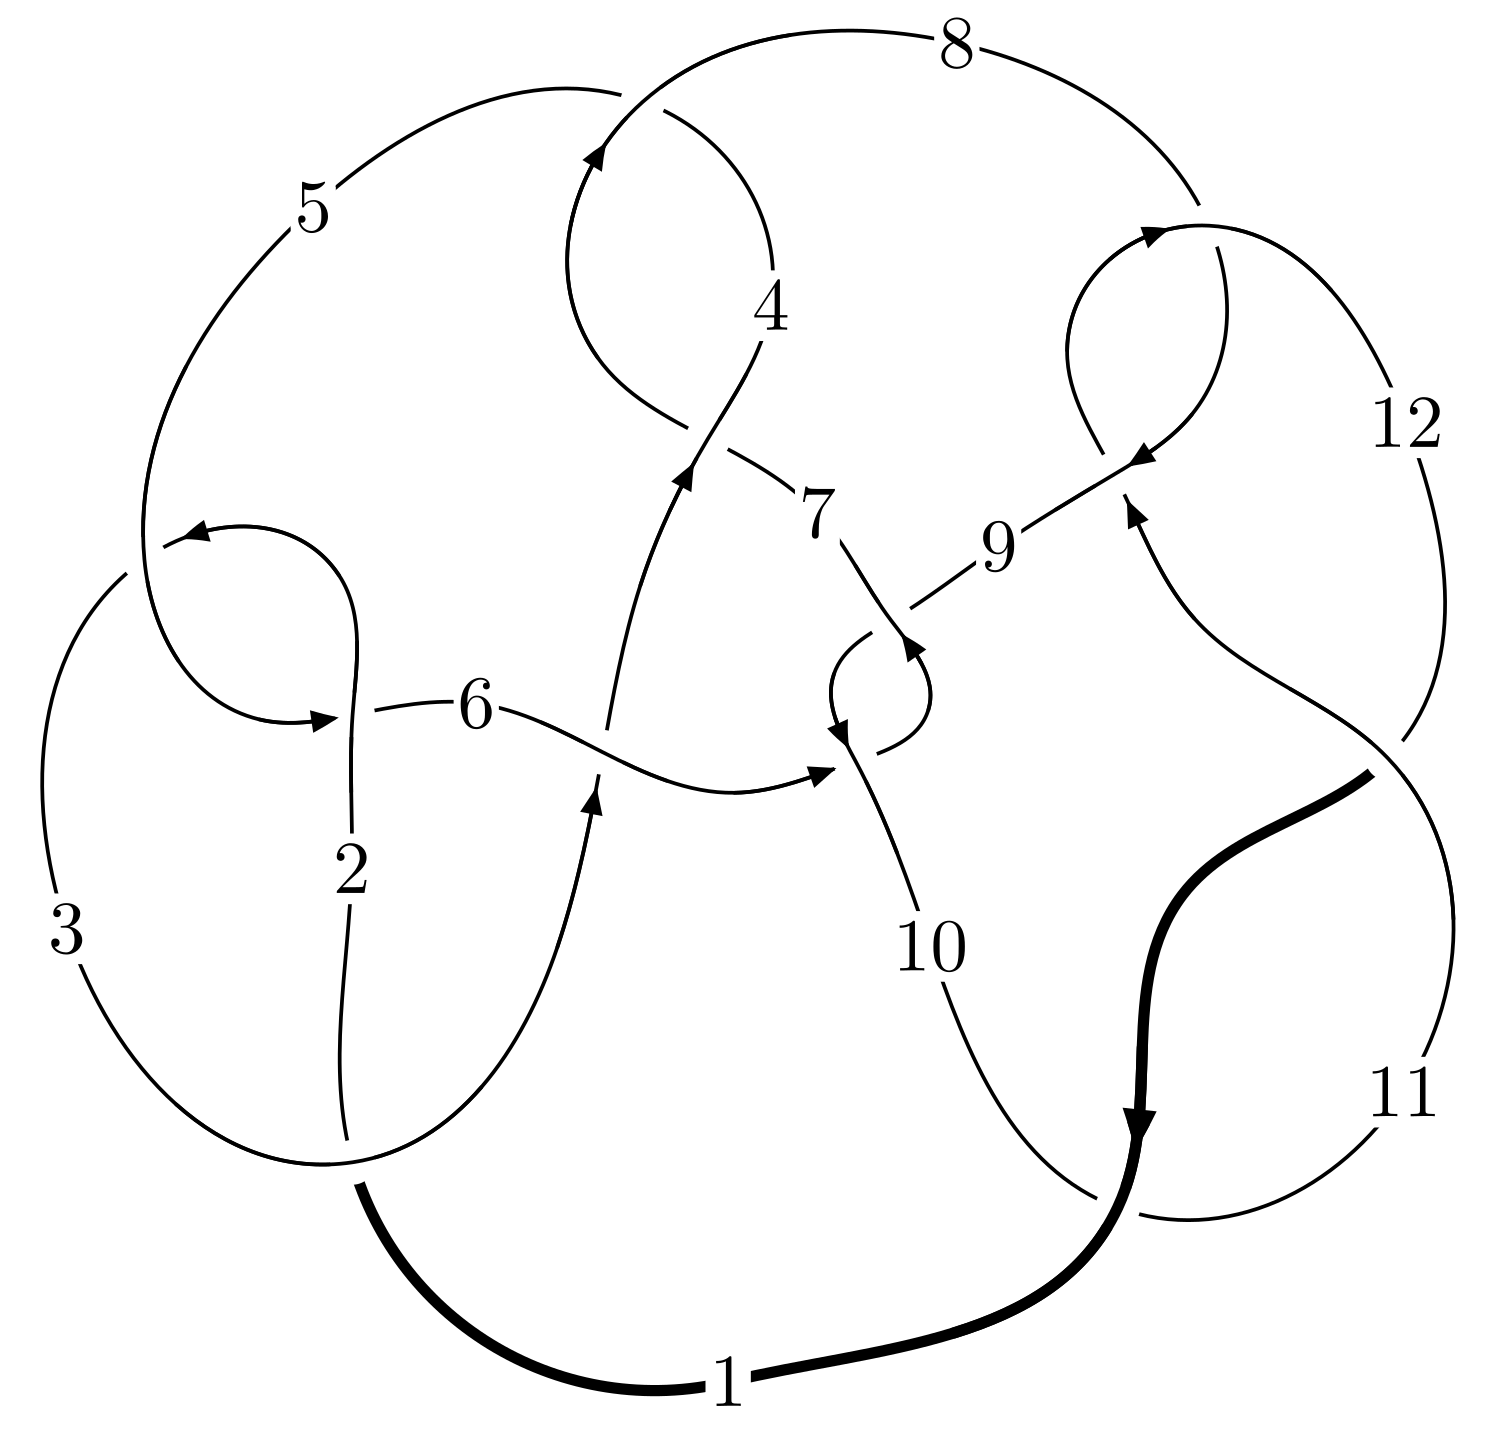
\includegraphics[width=112pt]{../../../GIT/diagram.site/Diagrams/png/806_12a_0005.png}\\
\ \ \ A knot diagram\footnotemark}&
\allowdisplaybreaks
\textbf{Linearized knot diagam} \\
\cline{2-2}
 &
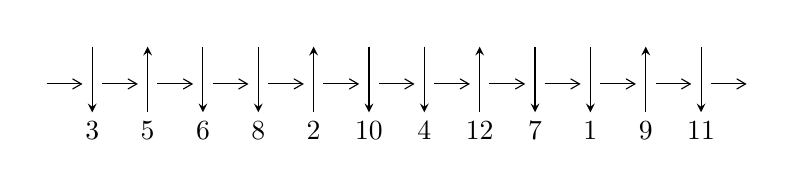
\begin{tikzpicture}[x=20pt, y=17pt]
	% nodes
	\node (C0) at (0, 0) {};
	\node (C1) at (1, 0) {};
	\node (C1U) at (1, +1) {};
	\node (C1D) at (1, -1) {3};

	\node (C2) at (2, 0) {};
	\node (C2U) at (2, +1) {};
	\node (C2D) at (2, -1) {5};

	\node (C3) at (3, 0) {};
	\node (C3U) at (3, +1) {};
	\node (C3D) at (3, -1) {6};

	\node (C4) at (4, 0) {};
	\node (C4U) at (4, +1) {};
	\node (C4D) at (4, -1) {8};

	\node (C5) at (5, 0) {};
	\node (C5U) at (5, +1) {};
	\node (C5D) at (5, -1) {2};

	\node (C6) at (6, 0) {};
	\node (C6U) at (6, +1) {};
	\node (C6D) at (6, -1) {10};

	\node (C7) at (7, 0) {};
	\node (C7U) at (7, +1) {};
	\node (C7D) at (7, -1) {4};

	\node (C8) at (8, 0) {};
	\node (C8U) at (8, +1) {};
	\node (C8D) at (8, -1) {12};

	\node (C9) at (9, 0) {};
	\node (C9U) at (9, +1) {};
	\node (C9D) at (9, -1) {7};

	\node (C10) at (10, 0) {};
	\node (C10U) at (10, +1) {};
	\node (C10D) at (10, -1) {1};

	\node (C11) at (11, 0) {};
	\node (C11U) at (11, +1) {};
	\node (C11D) at (11, -1) {9};

	\node (C12) at (12, 0) {};
	\node (C12U) at (12, +1) {};
	\node (C12D) at (12, -1) {11};
	\node (C13) at (13, 0) {};

	% arrows
	\draw[->,>={angle 60}]
	(C0) edge (C1) (C1) edge (C2) (C2) edge (C3) (C3) edge (C4) (C4) edge (C5) (C5) edge (C6) (C6) edge (C7) (C7) edge (C8) (C8) edge (C9) (C9) edge (C10) (C10) edge (C11) (C11) edge (C12) (C12) edge (C13) ;	\draw[->,>=stealth]
	(C1U) edge (C1D) (C2D) edge (C2U) (C3U) edge (C3D) (C4U) edge (C4D) (C5D) edge (C5U) (C6U) edge (C6D) (C7U) edge (C7D) (C8D) edge (C8U) (C9U) edge (C9D) (C10U) edge (C10D) (C11D) edge (C11U) (C12U) edge (C12D) ;
	\end{tikzpicture} \\
\hhline{~~} \\& 
\textbf{Solving Sequence} \\ \cline{2-2} 
 &
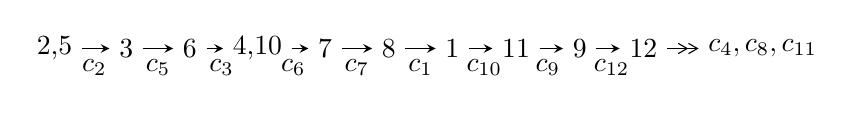
\begin{tikzpicture}[x=23pt, y=7pt]
	% node
	\node (A0) at (-1/8, 0) {2,5};
	\node (A1) at (1, 0) {3};
	\node (A2) at (2, 0) {6};
	\node (A3) at (49/16, 0) {4,10};
	\node (A4) at (33/8, 0) {7};
	\node (A5) at (41/8, 0) {8};
	\node (A6) at (49/8, 0) {1};
	\node (A7) at (57/8, 0) {11};
	\node (A8) at (65/8, 0) {9};
	\node (A9) at (73/8, 0) {12};
	\node (C1) at (1/2, -1) {$c_{2}$};
	\node (C2) at (3/2, -1) {$c_{5}$};
	\node (C3) at (5/2, -1) {$c_{3}$};
	\node (C4) at (29/8, -1) {$c_{6}$};
	\node (C5) at (37/8, -1) {$c_{7}$};
	\node (C6) at (45/8, -1) {$c_{1}$};
	\node (C7) at (53/8, -1) {$c_{10}$};
	\node (C8) at (61/8, -1) {$c_{9}$};
	\node (C9) at (69/8, -1) {$c_{12}$};
	\node (A10) at (11, 0) {$c_{4},c_{8},c_{11}$};

	% edge
	\draw[->,>=stealth]	
	(A0) edge (A1) (A1) edge (A2) (A2) edge (A3) (A3) edge (A4) (A4) edge (A5) (A5) edge (A6) (A6) edge (A7) (A7) edge (A8) (A8) edge (A9) ;
	\draw[->>,>={angle 60}]	
	(A9) edge (A10);
\end{tikzpicture} \\ 

\end{tabular} \\

\footnotetext{
The image of knot diagram is generated by the software ``\textbf{Draw programme}" developed by Andrew Bartholomew(\url{http://www.layer8.co.uk/maths/draw/index.htm\#Running-draw}), where we modified some parts for our purpose(\url{https://github.com/CATsTAILs/LinksPainter}).
}\phantom \\ \newline 
\centering \textbf{Ideals for irreducible components\footnotemark of $X_{\text{par}}$} 
 
\begin{align*}
I^u_{1}&=\langle 
-3.83259\times10^{67} u^{116}-1.82204\times10^{70} u^{115}+\cdots+8.69873\times10^{68} b+1.33324\times10^{70},\\
\phantom{I^u_{1}}&\phantom{= \langle  }1.23817\times10^{66} u^{116}-2.75088\times10^{67} u^{115}+\cdots+1.86668\times10^{66} a+2.43651\times10^{67},\;u^{117}-7 u^{116}+\cdots+2 u-1\rangle \\
I^u_{2}&=\langle 
b- a,\;- u^4 a+u^3 a-2 u^4- u^2 a+2 u^3+a^2-2 u^2+a- u+2,\;u^5- u^4+2 u^3- u^2+u-1\rangle \\
I^u_{3}&=\langle 
a^3 u+a^3-2 a^2-3 a u+b- a+u+1,\;a^4+2 a^3 u-3 a^2 u-3 a^2+a+u,\;u^2+u+1\rangle \\
\\
\end{align*}
\raggedright * 3 irreducible components of $\dim_{\mathbb{C}}=0$, with total 135 representations.\\
\footnotetext{All coefficients of polynomials are rational numbers. But the coefficients are sometimes approximated in decimal forms when there is not enough margin.}
\newpage
\renewcommand{\arraystretch}{1}
\centering \section*{I. $I^u_{1}= \langle -3.83\times10^{67} u^{116}-1.82\times10^{70} u^{115}+\cdots+8.70\times10^{68} b+1.33\times10^{70},\;1.24\times10^{66} u^{116}-2.75\times10^{67} u^{115}+\cdots+1.87\times10^{66} a+2.44\times10^{67},\;u^{117}-7 u^{116}+\cdots+2 u-1 \rangle$}
\flushleft \textbf{(i) Arc colorings}\\
\begin{tabular}{m{7pt} m{180pt} m{7pt} m{180pt} }
\flushright $a_{2}=$&$\begin{pmatrix}1\\0\end{pmatrix}$ \\
\flushright $a_{5}=$&$\begin{pmatrix}0\\u\end{pmatrix}$ \\
\flushright $a_{3}=$&$\begin{pmatrix}1\\- u^2\end{pmatrix}$ \\
\flushright $a_{6}=$&$\begin{pmatrix}u\\u\end{pmatrix}$ \\
\flushright $a_{4}=$&$\begin{pmatrix}u^4+u^2+1\\u^4\end{pmatrix}$ \\
\flushright $a_{10}=$&$\begin{pmatrix}-0.663298 u^{116}+14.7367 u^{115}+\cdots+13.8589 u-13.0526\\0.0440592 u^{116}+20.9461 u^{115}+\cdots+23.6452 u-15.3268\end{pmatrix}$ \\
\flushright $a_{7}=$&$\begin{pmatrix}2.35575 u^{116}-24.2437 u^{115}+\cdots-23.3034 u+10.4991\\5.54126 u^{116}-59.4144 u^{115}+\cdots-31.4570 u+17.5214\end{pmatrix}$ \\
\flushright $a_{8}=$&$\begin{pmatrix}-0.226928 u^{116}-3.84631 u^{115}+\cdots-16.0087 u+7.28280\\9.37936 u^{116}-80.9730 u^{115}+\cdots-36.3781 u+19.4890\end{pmatrix}$ \\
\flushright $a_{1}=$&$\begin{pmatrix}u^2+1\\- u^4\end{pmatrix}$ \\
\flushright $a_{11}=$&$\begin{pmatrix}-0.645907 u^{116}+15.9064 u^{115}+\cdots+11.8738 u-13.0533\\-0.477605 u^{116}+28.9600 u^{115}+\cdots+28.1091 u-17.8115\end{pmatrix}$ \\
\flushright $a_{9}=$&$\begin{pmatrix}-1.40166 u^{116}+21.6224 u^{115}+\cdots+23.6425 u-15.1337\\-3.20159 u^{116}+49.5014 u^{115}+\cdots+34.8907 u-20.7044\end{pmatrix}$ \\
\flushright $a_{12}=$&$\begin{pmatrix}-1.10727 u^{116}+8.57956 u^{115}+\cdots+12.9847 u-2.44428\\2.05987 u^{116}-13.3894 u^{115}+\cdots-1.35478 u+2.83905\end{pmatrix}$\\&\end{tabular}
\flushleft \textbf{(ii) Obstruction class $= -1$}\\~\\
\flushleft \textbf{(iii) Cusp Shapes $= -17.0712 u^{116}+107.696 u^{115}+\cdots-8.94784 u-8.30782$}\\~\\
\newpage\renewcommand{\arraystretch}{1}
\flushleft \textbf{(iv) u-Polynomials at the component}\newline \\
\begin{tabular}{m{50pt}|m{274pt}}
Crossings & \hspace{64pt}u-Polynomials at each crossing \\
\hline $$\begin{aligned}c_{1}\end{aligned}$$&$\begin{aligned}
&u^{117}+57 u^{116}+\cdots-52 u-1
\end{aligned}$\\
\hline $$\begin{aligned}c_{2},c_{5}\end{aligned}$$&$\begin{aligned}
&u^{117}+7 u^{116}+\cdots+2 u+1
\end{aligned}$\\
\hline $$\begin{aligned}c_{3}\end{aligned}$$&$\begin{aligned}
&u^{117}-7 u^{116}+\cdots-2123180 u+148289
\end{aligned}$\\
\hline $$\begin{aligned}c_{4},c_{7}\end{aligned}$$&$\begin{aligned}
&u^{117}+3 u^{116}+\cdots+384 u+256
\end{aligned}$\\
\hline $$\begin{aligned}c_{6},c_{9}\end{aligned}$$&$\begin{aligned}
&u^{117}-3 u^{116}+\cdots-6144 u+1024
\end{aligned}$\\
\hline $$\begin{aligned}c_{8},c_{11}\end{aligned}$$&$\begin{aligned}
&u^{117}+8 u^{116}+\cdots+5 u+1
\end{aligned}$\\
\hline $$\begin{aligned}c_{10},c_{12}\end{aligned}$$&$\begin{aligned}
&u^{117}+38 u^{116}+\cdots-199 u-1
\end{aligned}$\\
\hline
\end{tabular}\\~\\
\newpage\renewcommand{\arraystretch}{1}
\flushleft \textbf{(v) Riley Polynomials at the component}\newline \\
\begin{tabular}{m{50pt}|m{274pt}}
Crossings & \hspace{64pt}Riley Polynomials at each crossing \\
\hline $$\begin{aligned}c_{1}\end{aligned}$$&$\begin{aligned}
&y^{117}+13 y^{116}+\cdots-1116 y-1
\end{aligned}$\\
\hline $$\begin{aligned}c_{2},c_{5}\end{aligned}$$&$\begin{aligned}
&y^{117}+57 y^{116}+\cdots-52 y-1
\end{aligned}$\\
\hline $$\begin{aligned}c_{3}\end{aligned}$$&$\begin{aligned}
&y^{117}-31 y^{116}+\cdots-741103690564 y-21989627521
\end{aligned}$\\
\hline $$\begin{aligned}c_{4},c_{7}\end{aligned}$$&$\begin{aligned}
&y^{117}-55 y^{116}+\cdots+245760 y-65536
\end{aligned}$\\
\hline $$\begin{aligned}c_{6},c_{9}\end{aligned}$$&$\begin{aligned}
&y^{117}+65 y^{116}+\cdots-33554432 y-1048576
\end{aligned}$\\
\hline $$\begin{aligned}c_{8},c_{11}\end{aligned}$$&$\begin{aligned}
&y^{117}+38 y^{116}+\cdots-199 y-1
\end{aligned}$\\
\hline $$\begin{aligned}c_{10},c_{12}\end{aligned}$$&$\begin{aligned}
&y^{117}+90 y^{116}+\cdots+15017 y-1
\end{aligned}$\\
\hline
\end{tabular}\\~\\
\newpage\flushleft \textbf{(vi) Complex Volumes and Cusp Shapes}
$$\begin{array}{c|c|c}  
\text{Solutions to }I^u_{1}& \I (\text{vol} + \sqrt{-1}CS) & \text{Cusp shape}\\
 \hline 
\begin{aligned}
u &= -0.788050 + 0.643963 I \\
a &= \phantom{-}0.441133 - 0.436719 I \\
b &= -0.030091 + 0.782506 I\end{aligned}
 & \phantom{-}6.38871 - 3.43951 I & \phantom{-0.000000 } 0 \\ \hline\begin{aligned}
u &= -0.788050 - 0.643963 I \\
a &= \phantom{-}0.441133 + 0.436719 I \\
b &= -0.030091 - 0.782506 I\end{aligned}
 & \phantom{-}6.38871 + 3.43951 I & \phantom{-0.000000 } 0 \\ \hline\begin{aligned}
u &= -0.436106 + 0.936175 I \\
a &= \phantom{-}0.78008 + 3.14764 I \\
b &= \phantom{-}0.51824 + 3.56972 I\end{aligned}
 & -0.482514 + 0.107557 I & \phantom{-0.000000 } 0 \\ \hline\begin{aligned}
u &= -0.436106 - 0.936175 I \\
a &= \phantom{-}0.78008 - 3.14764 I \\
b &= \phantom{-}0.51824 - 3.56972 I\end{aligned}
 & -0.482514 - 0.107557 I & \phantom{-0.000000 } 0 \\ \hline\begin{aligned}
u &= -0.650362 + 0.706698 I \\
a &= -0.958278 - 0.474899 I \\
b &= -0.59593 - 1.35751 I\end{aligned}
 & -0.40559 - 4.29098 I & \phantom{-0.000000 } 0 \\ \hline\begin{aligned}
u &= -0.650362 - 0.706698 I \\
a &= -0.958278 + 0.474899 I \\
b &= -0.59593 + 1.35751 I\end{aligned}
 & -0.40559 + 4.29098 I & \phantom{-0.000000 } 0 \\ \hline\begin{aligned}
u &= -0.459329 + 0.839596 I \\
a &= -2.18263 - 3.06586 I \\
b &= -1.97132 - 3.38773 I\end{aligned}
 & -0.15385 - 3.78902 I & \phantom{-0.000000 } 0 \\ \hline\begin{aligned}
u &= -0.459329 - 0.839596 I \\
a &= -2.18263 + 3.06586 I \\
b &= -1.97132 + 3.38773 I\end{aligned}
 & -0.15385 + 3.78902 I & \phantom{-0.000000 } 0 \\ \hline\begin{aligned}
u &= -0.795690 + 0.676627 I \\
a &= -0.258135 + 0.303256 I \\
b &= \phantom{-}0.139411 - 0.928846 I\end{aligned}
 & \phantom{-}5.60113 - 9.33628 I & \phantom{-0.000000 } 0 \\ \hline\begin{aligned}
u &= -0.795690 - 0.676627 I \\
a &= -0.258135 - 0.303256 I \\
b &= \phantom{-}0.139411 + 0.928846 I\end{aligned}
 & \phantom{-}5.60113 + 9.33628 I & \phantom{-0.000000 } 0\\
 \hline 
 \end{array}$$\newpage$$\begin{array}{c|c|c}  
\text{Solutions to }I^u_{1}& \I (\text{vol} + \sqrt{-1}CS) & \text{Cusp shape}\\
 \hline 
\begin{aligned}
u &= -0.622734 + 0.853712 I \\
a &= \phantom{-}1.130780 + 0.426011 I \\
b &= \phantom{-}0.368893 + 0.451916 I\end{aligned}
 & -0.816274 - 0.627025 I & \phantom{-0.000000 } 0 \\ \hline\begin{aligned}
u &= -0.622734 - 0.853712 I \\
a &= \phantom{-}1.130780 - 0.426011 I \\
b &= \phantom{-}0.368893 - 0.451916 I\end{aligned}
 & -0.816274 + 0.627025 I & \phantom{-0.000000 } 0 \\ \hline\begin{aligned}
u &= -0.387152 + 0.859674 I \\
a &= \phantom{-}0.438751 - 0.612774 I \\
b &= \phantom{-}0.142021 - 0.759816 I\end{aligned}
 & -0.34124 - 1.65771 I & \phantom{-0.000000 } 0 \\ \hline\begin{aligned}
u &= -0.387152 - 0.859674 I \\
a &= \phantom{-}0.438751 + 0.612774 I \\
b &= \phantom{-}0.142021 + 0.759816 I\end{aligned}
 & -0.34124 + 1.65771 I & \phantom{-0.000000 } 0 \\ \hline\begin{aligned}
u &= \phantom{-}0.863128 + 0.357713 I \\
a &= -1.87347 - 0.80598 I \\
b &= -0.646595 + 0.167847 I\end{aligned}
 & \phantom{-}3.70909 - 12.80720 I & \phantom{-0.000000 } 0 \\ \hline\begin{aligned}
u &= \phantom{-}0.863128 - 0.357713 I \\
a &= -1.87347 + 0.80598 I \\
b &= -0.646595 - 0.167847 I\end{aligned}
 & \phantom{-}3.70909 + 12.80720 I & \phantom{-0.000000 } 0 \\ \hline\begin{aligned}
u &= \phantom{-}0.842943 + 0.374277 I \\
a &= \phantom{-}1.75421 + 0.78574 I \\
b &= \phantom{-}0.544568 - 0.230616 I\end{aligned}
 & \phantom{-}4.83595 - 6.78698 I & \phantom{-0.000000 } 0 \\ \hline\begin{aligned}
u &= \phantom{-}0.842943 - 0.374277 I \\
a &= \phantom{-}1.75421 - 0.78574 I \\
b &= \phantom{-}0.544568 + 0.230616 I\end{aligned}
 & \phantom{-}4.83595 + 6.78698 I & \phantom{-0.000000 } 0 \\ \hline\begin{aligned}
u &= \phantom{-}0.259158 + 1.065270 I \\
a &= \phantom{-}0.375121 + 0.409369 I \\
b &= -0.662192 + 0.708860 I\end{aligned}
 & -2.20289 - 1.03572 I & \phantom{-0.000000 } 0 \\ \hline\begin{aligned}
u &= \phantom{-}0.259158 - 1.065270 I \\
a &= \phantom{-}0.375121 - 0.409369 I \\
b &= -0.662192 - 0.708860 I\end{aligned}
 & -2.20289 + 1.03572 I & \phantom{-0.000000 } 0\\
 \hline 
 \end{array}$$\newpage$$\begin{array}{c|c|c}  
\text{Solutions to }I^u_{1}& \I (\text{vol} + \sqrt{-1}CS) & \text{Cusp shape}\\
 \hline 
\begin{aligned}
u &= \phantom{-}0.495668 + 0.977957 I \\
a &= \phantom{-}0.395468 - 0.391923 I \\
b &= -1.047470 - 0.895669 I\end{aligned}
 & \phantom{-}6.56810 - 0.57006 I & \phantom{-0.000000 } 0 \\ \hline\begin{aligned}
u &= \phantom{-}0.495668 - 0.977957 I \\
a &= \phantom{-}0.395468 + 0.391923 I \\
b &= -1.047470 + 0.895669 I\end{aligned}
 & \phantom{-}6.56810 + 0.57006 I & \phantom{-0.000000 } 0 \\ \hline\begin{aligned}
u &= \phantom{-}0.291276 + 1.064330 I \\
a &= -0.066879 + 1.287670 I \\
b &= \phantom{-}0.18397 + 2.32609 I\end{aligned}
 & -2.46003 + 2.02278 I & \phantom{-0.000000 } 0 \\ \hline\begin{aligned}
u &= \phantom{-}0.291276 - 1.064330 I \\
a &= -0.066879 - 1.287670 I \\
b &= \phantom{-}0.18397 - 2.32609 I\end{aligned}
 & -2.46003 - 2.02278 I & \phantom{-0.000000 } 0 \\ \hline\begin{aligned}
u &= \phantom{-}0.887934 + 0.028589 I \\
a &= -0.175661 + 1.187160 I \\
b &= -0.064609 + 0.239852 I\end{aligned}
 & -1.47278 + 2.54621 I & \phantom{-0.000000 } 0 \\ \hline\begin{aligned}
u &= \phantom{-}0.887934 - 0.028589 I \\
a &= -0.175661 - 1.187160 I \\
b &= -0.064609 - 0.239852 I\end{aligned}
 & -1.47278 - 2.54621 I & \phantom{-0.000000 } 0 \\ \hline\begin{aligned}
u &= \phantom{-}0.520884 + 0.991503 I \\
a &= -0.319131 + 0.493403 I \\
b &= \phantom{-}1.02158 + 1.13380 I\end{aligned}
 & \phantom{-}6.78221 + 5.92923 I & \phantom{-0.000000 } 0 \\ \hline\begin{aligned}
u &= \phantom{-}0.520884 - 0.991503 I \\
a &= -0.319131 - 0.493403 I \\
b &= \phantom{-}1.02158 - 1.13380 I\end{aligned}
 & \phantom{-}6.78221 - 5.92923 I & \phantom{-0.000000 } 0 \\ \hline\begin{aligned}
u &= -0.558143 + 0.981636 I \\
a &= \phantom{-}0.06180 - 1.84492 I \\
b &= -0.36559 - 2.44954 I\end{aligned}
 & \phantom{-}0.918923 - 0.592170 I & \phantom{-0.000000 } 0 \\ \hline\begin{aligned}
u &= -0.558143 - 0.981636 I \\
a &= \phantom{-}0.06180 + 1.84492 I \\
b &= -0.36559 + 2.44954 I\end{aligned}
 & \phantom{-}0.918923 + 0.592170 I & \phantom{-0.000000 } 0\\
 \hline 
 \end{array}$$\newpage$$\begin{array}{c|c|c}  
\text{Solutions to }I^u_{1}& \I (\text{vol} + \sqrt{-1}CS) & \text{Cusp shape}\\
 \hline 
\begin{aligned}
u &= \phantom{-}0.241670 + 1.106980 I \\
a &= -0.03421 - 1.53422 I \\
b &= -0.36187 - 2.52798 I\end{aligned}
 & -3.52324 - 3.49244 I & \phantom{-0.000000 } 0 \\ \hline\begin{aligned}
u &= \phantom{-}0.241670 - 1.106980 I \\
a &= -0.03421 + 1.53422 I \\
b &= -0.36187 + 2.52798 I\end{aligned}
 & -3.52324 + 3.49244 I & \phantom{-0.000000 } 0 \\ \hline\begin{aligned}
u &= -0.636348 + 0.587639 I \\
a &= \phantom{-}1.65981 + 0.37698 I \\
b &= \phantom{-}0.754385 - 0.268951 I\end{aligned}
 & \phantom{-}2.08032 - 4.09466 I & \phantom{-0.000000 } 0 \\ \hline\begin{aligned}
u &= -0.636348 - 0.587639 I \\
a &= \phantom{-}1.65981 - 0.37698 I \\
b &= \phantom{-}0.754385 + 0.268951 I\end{aligned}
 & \phantom{-}2.08032 + 4.09466 I & \phantom{-0.000000 } 0 \\ \hline\begin{aligned}
u &= -0.402200 + 1.067810 I \\
a &= \phantom{-}0.43074 + 1.47123 I \\
b &= \phantom{-}1.16303 + 1.75138 I\end{aligned}
 & -2.93679 - 1.28935 I & \phantom{-0.000000 } 0 \\ \hline\begin{aligned}
u &= -0.402200 - 1.067810 I \\
a &= \phantom{-}0.43074 - 1.47123 I \\
b &= \phantom{-}1.16303 - 1.75138 I\end{aligned}
 & -2.93679 + 1.28935 I & \phantom{-0.000000 } 0 \\ \hline\begin{aligned}
u &= \phantom{-}0.331096 + 1.100150 I \\
a &= -0.854097 - 0.483958 I \\
b &= \phantom{-}0.097301 - 0.669536 I\end{aligned}
 & -4.41468 + 3.80335 I & \phantom{-0.000000 } 0 \\ \hline\begin{aligned}
u &= \phantom{-}0.331096 - 1.100150 I \\
a &= -0.854097 + 0.483958 I \\
b &= \phantom{-}0.097301 + 0.669536 I\end{aligned}
 & -4.41468 - 3.80335 I & \phantom{-0.000000 } 0 \\ \hline\begin{aligned}
u &= \phantom{-}0.788143 + 0.307476 I \\
a &= -1.78183 - 0.40923 I \\
b &= -0.723918 + 0.564808 I\end{aligned}
 & -2.40584 - 6.41831 I & \phantom{-0.000000 } 0 \\ \hline\begin{aligned}
u &= \phantom{-}0.788143 - 0.307476 I \\
a &= -1.78183 + 0.40923 I \\
b &= -0.723918 - 0.564808 I\end{aligned}
 & -2.40584 + 6.41831 I & \phantom{-0.000000 } 0\\
 \hline 
 \end{array}$$\newpage$$\begin{array}{c|c|c}  
\text{Solutions to }I^u_{1}& \I (\text{vol} + \sqrt{-1}CS) & \text{Cusp shape}\\
 \hline 
\begin{aligned}
u &= \phantom{-}0.597169 + 0.597551 I \\
a &= \phantom{-}0.836553 + 0.317154 I \\
b &= -0.300337 - 1.081280 I\end{aligned}
 & \phantom{-}7.95045 - 1.49171 I & \phantom{-0.000000 } 0 \\ \hline\begin{aligned}
u &= \phantom{-}0.597169 - 0.597551 I \\
a &= \phantom{-}0.836553 - 0.317154 I \\
b &= -0.300337 + 1.081280 I\end{aligned}
 & \phantom{-}7.95045 + 1.49171 I & \phantom{-0.000000 } 0 \\ \hline\begin{aligned}
u &= -0.562393 + 1.012380 I \\
a &= -0.04278 - 1.50341 I \\
b &= \phantom{-}0.59004 - 2.01129 I\end{aligned}
 & \phantom{-}1.40553 - 3.26753 I & \phantom{-0.000000 } 0 \\ \hline\begin{aligned}
u &= -0.562393 - 1.012380 I \\
a &= -0.04278 + 1.50341 I \\
b &= \phantom{-}0.59004 + 2.01129 I\end{aligned}
 & \phantom{-}1.40553 + 3.26753 I & \phantom{-0.000000 } 0 \\ \hline\begin{aligned}
u &= \phantom{-}0.552045 + 0.635041 I \\
a &= -0.777686 - 0.173295 I \\
b &= \phantom{-}0.343721 + 1.274540 I\end{aligned}
 & \phantom{-}7.59257 + 4.78397 I & \phantom{-0.000000 } 0 \\ \hline\begin{aligned}
u &= \phantom{-}0.552045 - 0.635041 I \\
a &= -0.777686 + 0.173295 I \\
b &= \phantom{-}0.343721 - 1.274540 I\end{aligned}
 & \phantom{-}7.59257 - 4.78397 I & \phantom{-0.000000 } 0 \\ \hline\begin{aligned}
u &= -0.642479 + 0.537916 I \\
a &= \phantom{-}1.50891 - 0.45918 I \\
b &= \phantom{-}0.760280 + 0.486993 I\end{aligned}
 & \phantom{-}2.80307 - 1.45282 I & \phantom{-0.000000 } 0 \\ \hline\begin{aligned}
u &= -0.642479 - 0.537916 I \\
a &= \phantom{-}1.50891 + 0.45918 I \\
b &= \phantom{-}0.760280 - 0.486993 I\end{aligned}
 & \phantom{-}2.80307 + 1.45282 I & \phantom{-0.000000 } 0 \\ \hline\begin{aligned}
u &= -0.241010 + 1.137390 I \\
a &= -0.994770 - 0.885964 I \\
b &= -1.94230 - 0.88243 I\end{aligned}
 & \phantom{-}2.14923 - 2.38133 I & \phantom{-0.000000 } 0 \\ \hline\begin{aligned}
u &= -0.241010 - 1.137390 I \\
a &= -0.994770 + 0.885964 I \\
b &= -1.94230 + 0.88243 I\end{aligned}
 & \phantom{-}2.14923 + 2.38133 I & \phantom{-0.000000 } 0\\
 \hline 
 \end{array}$$\newpage$$\begin{array}{c|c|c}  
\text{Solutions to }I^u_{1}& \I (\text{vol} + \sqrt{-1}CS) & \text{Cusp shape}\\
 \hline 
\begin{aligned}
u &= -0.536282 + 1.031720 I \\
a &= \phantom{-}0.03646 + 1.86790 I \\
b &= \phantom{-}0.60835 + 2.44313 I\end{aligned}
 & \phantom{-}0.57777 - 5.74969 I & \phantom{-0.000000 } 0 \\ \hline\begin{aligned}
u &= -0.536282 - 1.031720 I \\
a &= \phantom{-}0.03646 - 1.86790 I \\
b &= \phantom{-}0.60835 - 2.44313 I\end{aligned}
 & \phantom{-}0.57777 + 5.74969 I & \phantom{-0.000000 } 0 \\ \hline\begin{aligned}
u &= -0.749091 + 0.335717 I \\
a &= \phantom{-}1.67621 - 1.39851 I \\
b &= \phantom{-}0.630951 - 0.165919 I\end{aligned}
 & \phantom{-}6.64713 + 0.36834 I & \phantom{-0.000000 } 0 \\ \hline\begin{aligned}
u &= -0.749091 - 0.335717 I \\
a &= \phantom{-}1.67621 + 1.39851 I \\
b &= \phantom{-}0.630951 + 0.165919 I\end{aligned}
 & \phantom{-}6.64713 - 0.36834 I & \phantom{-0.000000 } 0 \\ \hline\begin{aligned}
u &= \phantom{-}0.743090 + 0.344565 I \\
a &= -1.37666 + 0.62863 I \\
b &= -0.296731 - 0.415869 I\end{aligned}
 & \phantom{-}0.90323 - 6.10586 I & \phantom{-0.000000 } 0 \\ \hline\begin{aligned}
u &= \phantom{-}0.743090 - 0.344565 I \\
a &= -1.37666 - 0.62863 I \\
b &= -0.296731 + 0.415869 I\end{aligned}
 & \phantom{-}0.90323 + 6.10586 I & \phantom{-0.000000 } 0 \\ \hline\begin{aligned}
u &= -0.498147 + 1.077050 I \\
a &= -0.51304 + 2.12295 I \\
b &= -1.01752 + 2.82627 I\end{aligned}
 & -2.25240 - 5.67314 I & \phantom{-0.000000 } 0 \\ \hline\begin{aligned}
u &= -0.498147 - 1.077050 I \\
a &= -0.51304 - 2.12295 I \\
b &= -1.01752 - 2.82627 I\end{aligned}
 & -2.25240 + 5.67314 I & \phantom{-0.000000 } 0 \\ \hline\begin{aligned}
u &= -0.286372 + 1.155600 I \\
a &= \phantom{-}1.03487 + 1.11825 I \\
b &= \phantom{-}1.99849 + 1.20360 I\end{aligned}
 & \phantom{-}1.61709 + 3.18256 I & \phantom{-0.000000 } 0 \\ \hline\begin{aligned}
u &= -0.286372 - 1.155600 I \\
a &= \phantom{-}1.03487 - 1.11825 I \\
b &= \phantom{-}1.99849 - 1.20360 I\end{aligned}
 & \phantom{-}1.61709 - 3.18256 I & \phantom{-0.000000 } 0\\
 \hline 
 \end{array}$$\newpage$$\begin{array}{c|c|c}  
\text{Solutions to }I^u_{1}& \I (\text{vol} + \sqrt{-1}CS) & \text{Cusp shape}\\
 \hline 
\begin{aligned}
u &= \phantom{-}0.242947 + 1.167530 I \\
a &= -0.213044 - 1.030830 I \\
b &= \phantom{-}0.73246 - 1.40141 I\end{aligned}
 & -7.04923 - 3.39820 I & \phantom{-0.000000 } 0 \\ \hline\begin{aligned}
u &= \phantom{-}0.242947 - 1.167530 I \\
a &= -0.213044 + 1.030830 I \\
b &= \phantom{-}0.73246 + 1.40141 I\end{aligned}
 & -7.04923 + 3.39820 I & \phantom{-0.000000 } 0 \\ \hline\begin{aligned}
u &= -0.751272 + 0.284916 I \\
a &= -1.80885 + 1.49561 I \\
b &= -0.698513 + 0.241621 I\end{aligned}
 & \phantom{-}5.93364 + 6.27192 I & \phantom{-0.000000 } 0 \\ \hline\begin{aligned}
u &= -0.751272 - 0.284916 I \\
a &= -1.80885 - 1.49561 I \\
b &= -0.698513 - 0.241621 I\end{aligned}
 & \phantom{-}5.93364 - 6.27192 I & \phantom{-0.000000 } 0 \\ \hline\begin{aligned}
u &= -0.714184 + 0.960943 I \\
a &= \phantom{-}0.217324 + 0.091526 I \\
b &= -0.810052 + 0.410513 I\end{aligned}
 & \phantom{-}4.75806 + 3.70162 I & \phantom{-0.000000 } 0 \\ \hline\begin{aligned}
u &= -0.714184 - 0.960943 I \\
a &= \phantom{-}0.217324 - 0.091526 I \\
b &= -0.810052 - 0.410513 I\end{aligned}
 & \phantom{-}4.75806 - 3.70162 I & \phantom{-0.000000 } 0 \\ \hline\begin{aligned}
u &= \phantom{-}0.714416 + 0.366021 I \\
a &= \phantom{-}1.43841 + 0.41582 I \\
b &= \phantom{-}0.399059 - 0.722002 I\end{aligned}
 & \phantom{-}2.01022 - 3.40590 I & \phantom{-0.000000 } 0 \\ \hline\begin{aligned}
u &= \phantom{-}0.714416 - 0.366021 I \\
a &= \phantom{-}1.43841 - 0.41582 I \\
b &= \phantom{-}0.399059 + 0.722002 I\end{aligned}
 & \phantom{-}2.01022 + 3.40590 I & \phantom{-0.000000 } 0 \\ \hline\begin{aligned}
u &= \phantom{-}0.784133 + 0.167033 I \\
a &= -0.946265 + 0.770926 I \\
b &= -0.220586 - 0.048660 I\end{aligned}
 & -4.22647 - 1.60861 I & \phantom{-0.000000 } 0 \\ \hline\begin{aligned}
u &= \phantom{-}0.784133 - 0.167033 I \\
a &= -0.946265 - 0.770926 I \\
b &= -0.220586 + 0.048660 I\end{aligned}
 & -4.22647 + 1.60861 I & \phantom{-0.000000 } 0\\
 \hline 
 \end{array}$$\newpage$$\begin{array}{c|c|c}  
\text{Solutions to }I^u_{1}& \I (\text{vol} + \sqrt{-1}CS) & \text{Cusp shape}\\
 \hline 
\begin{aligned}
u &= -0.694981 + 0.982159 I \\
a &= -0.073453 - 0.271762 I \\
b &= \phantom{-}0.906822 - 0.651608 I\end{aligned}
 & \phantom{-}5.38630 - 2.11378 I & \phantom{-0.000000 } 0 \\ \hline\begin{aligned}
u &= -0.694981 - 0.982159 I \\
a &= -0.073453 + 0.271762 I \\
b &= \phantom{-}0.906822 + 0.651608 I\end{aligned}
 & \phantom{-}5.38630 + 2.11378 I & \phantom{-0.000000 } 0 \\ \hline\begin{aligned}
u &= \phantom{-}0.152478 + 1.194550 I \\
a &= -0.423715 + 0.926756 I \\
b &= -1.43935 + 1.33380 I\end{aligned}
 & -0.47338 - 3.99674 I & \phantom{-0.000000 } 0 \\ \hline\begin{aligned}
u &= \phantom{-}0.152478 - 1.194550 I \\
a &= -0.423715 - 0.926756 I \\
b &= -1.43935 - 1.33380 I\end{aligned}
 & -0.47338 + 3.99674 I & \phantom{-0.000000 } 0 \\ \hline\begin{aligned}
u &= \phantom{-}0.436147 + 1.131570 I \\
a &= \phantom{-}0.042081 + 0.819809 I \\
b &= -0.08366 + 1.52333 I\end{aligned}
 & -4.67639 + 3.90668 I & \phantom{-0.000000 } 0 \\ \hline\begin{aligned}
u &= \phantom{-}0.436147 - 1.131570 I \\
a &= \phantom{-}0.042081 - 0.819809 I \\
b &= -0.08366 - 1.52333 I\end{aligned}
 & -4.67639 - 3.90668 I & \phantom{-0.000000 } 0 \\ \hline\begin{aligned}
u &= -0.601257 + 0.504673 I \\
a &= -1.71238 - 0.62803 I \\
b &= -0.829199 + 0.215477 I\end{aligned}
 & \phantom{-}2.13316 + 1.22336 I & \phantom{-0.000000 } 0 \\ \hline\begin{aligned}
u &= -0.601257 - 0.504673 I \\
a &= -1.71238 + 0.62803 I \\
b &= -0.829199 - 0.215477 I\end{aligned}
 & \phantom{-}2.13316 - 1.22336 I & \phantom{-0.000000 } 0 \\ \hline\begin{aligned}
u &= \phantom{-}0.523972 + 1.106740 I \\
a &= \phantom{-}0.64089 - 1.39244 I \\
b &= -0.13170 - 1.98598 I\end{aligned}
 & -3.09840 + 3.62785 I & \phantom{-0.000000 } 0 \\ \hline\begin{aligned}
u &= \phantom{-}0.523972 - 1.106740 I \\
a &= \phantom{-}0.64089 + 1.39244 I \\
b &= -0.13170 + 1.98598 I\end{aligned}
 & -3.09840 - 3.62785 I & \phantom{-0.000000 } 0\\
 \hline 
 \end{array}$$\newpage$$\begin{array}{c|c|c}  
\text{Solutions to }I^u_{1}& \I (\text{vol} + \sqrt{-1}CS) & \text{Cusp shape}\\
 \hline 
\begin{aligned}
u &= \phantom{-}0.549843 + 1.100120 I \\
a &= -0.132774 + 1.076900 I \\
b &= -0.84858 + 1.88003 I\end{aligned}
 & -0.67169 + 5.16920 I & \phantom{-0.000000 } 0 \\ \hline\begin{aligned}
u &= \phantom{-}0.549843 - 1.100120 I \\
a &= -0.132774 - 1.076900 I \\
b &= -0.84858 - 1.88003 I\end{aligned}
 & -0.67169 - 5.16920 I & \phantom{-0.000000 } 0 \\ \hline\begin{aligned}
u &= \phantom{-}0.681708 + 0.356666 I \\
a &= \phantom{-}1.32997 - 0.53776 I \\
b &= \phantom{-}0.160489 + 0.459931 I\end{aligned}
 & \phantom{-}1.48482 - 0.40443 I & \phantom{-0.000000 } 0 \\ \hline\begin{aligned}
u &= \phantom{-}0.681708 - 0.356666 I \\
a &= \phantom{-}1.32997 + 0.53776 I \\
b &= \phantom{-}0.160489 - 0.459931 I\end{aligned}
 & \phantom{-}1.48482 + 0.40443 I & \phantom{-0.000000 } 0 \\ \hline\begin{aligned}
u &= \phantom{-}0.345072 + 1.184100 I \\
a &= -0.471587 - 1.087290 I \\
b &= -0.76488 - 1.84916 I\end{aligned}
 & -8.31174 + 2.09718 I & \phantom{-0.000000 } 0 \\ \hline\begin{aligned}
u &= \phantom{-}0.345072 - 1.184100 I \\
a &= -0.471587 + 1.087290 I \\
b &= -0.76488 + 1.84916 I\end{aligned}
 & -8.31174 - 2.09718 I & \phantom{-0.000000 } 0 \\ \hline\begin{aligned}
u &= \phantom{-}0.170264 + 1.223690 I \\
a &= \phantom{-}0.439760 - 1.157850 I \\
b &= \phantom{-}1.44857 - 1.59171 I\end{aligned}
 & -1.64372 - 9.78312 I & \phantom{-0.000000 } 0 \\ \hline\begin{aligned}
u &= \phantom{-}0.170264 - 1.223690 I \\
a &= \phantom{-}0.439760 + 1.157850 I \\
b &= \phantom{-}1.44857 + 1.59171 I\end{aligned}
 & -1.64372 + 9.78312 I & \phantom{-0.000000 } 0 \\ \hline\begin{aligned}
u &= \phantom{-}0.561453 + 1.104500 I \\
a &= -0.18042 + 1.42465 I \\
b &= \phantom{-}0.60353 + 2.19281 I\end{aligned}
 & -0.14818 + 8.29193 I & \phantom{-0.000000 } 0 \\ \hline\begin{aligned}
u &= \phantom{-}0.561453 - 1.104500 I \\
a &= -0.18042 - 1.42465 I \\
b &= \phantom{-}0.60353 - 2.19281 I\end{aligned}
 & -0.14818 - 8.29193 I & \phantom{-0.000000 } 0\\
 \hline 
 \end{array}$$\newpage$$\begin{array}{c|c|c}  
\text{Solutions to }I^u_{1}& \I (\text{vol} + \sqrt{-1}CS) & \text{Cusp shape}\\
 \hline 
\begin{aligned}
u &= \phantom{-}0.565539 + 1.117910 I \\
a &= \phantom{-}0.205821 - 1.138550 I \\
b &= \phantom{-}0.99445 - 1.86392 I\end{aligned}
 & -1.36213 + 11.07080 I & \phantom{-0.000000 } 0 \\ \hline\begin{aligned}
u &= \phantom{-}0.565539 - 1.117910 I \\
a &= \phantom{-}0.205821 + 1.138550 I \\
b &= \phantom{-}0.99445 + 1.86392 I\end{aligned}
 & -1.36213 - 11.07080 I & \phantom{-0.000000 } 0 \\ \hline\begin{aligned}
u &= -0.567660 + 1.120280 I \\
a &= \phantom{-}0.92774 - 1.58823 I \\
b &= \phantom{-}1.61984 - 2.36858 I\end{aligned}
 & \phantom{-}4.35518 - 5.35177 I & \phantom{-0.000000 } 0 \\ \hline\begin{aligned}
u &= -0.567660 - 1.120280 I \\
a &= \phantom{-}0.92774 + 1.58823 I \\
b &= \phantom{-}1.61984 + 2.36858 I\end{aligned}
 & \phantom{-}4.35518 + 5.35177 I & \phantom{-0.000000 } 0 \\ \hline\begin{aligned}
u &= -0.112035 + 0.733492 I \\
a &= -0.252312 - 0.649208 I \\
b &= -0.801580 + 0.061448 I\end{aligned}
 & -0.98803 - 1.33457 I & \phantom{-0.000000 } 0 \\ \hline\begin{aligned}
u &= -0.112035 - 0.733492 I \\
a &= -0.252312 + 0.649208 I \\
b &= -0.801580 - 0.061448 I\end{aligned}
 & -0.98803 + 1.33457 I & \phantom{-0.000000 } 0 \\ \hline\begin{aligned}
u &= -0.553058 + 1.137830 I \\
a &= -1.04926 + 1.73476 I \\
b &= -1.71134 + 2.56327 I\end{aligned}
 & \phantom{-}3.44904 - 11.19340 I & \phantom{-0.000000 } 0 \\ \hline\begin{aligned}
u &= -0.553058 - 1.137830 I \\
a &= -1.04926 - 1.73476 I \\
b &= -1.71134 - 2.56327 I\end{aligned}
 & \phantom{-}3.44904 + 11.19340 I & \phantom{-0.000000 } 0 \\ \hline\begin{aligned}
u &= \phantom{-}0.567903 + 1.141310 I \\
a &= \phantom{-}0.05003 - 1.87100 I \\
b &= -0.57280 - 2.68050 I\end{aligned}
 & -4.86384 + 11.49110 I & \phantom{-0.000000 } 0 \\ \hline\begin{aligned}
u &= \phantom{-}0.567903 - 1.141310 I \\
a &= \phantom{-}0.05003 + 1.87100 I \\
b &= -0.57280 + 2.68050 I\end{aligned}
 & -4.86384 - 11.49110 I & \phantom{-0.000000 } 0\\
 \hline 
 \end{array}$$\newpage$$\begin{array}{c|c|c}  
\text{Solutions to }I^u_{1}& \I (\text{vol} + \sqrt{-1}CS) & \text{Cusp shape}\\
 \hline 
\begin{aligned}
u &= \phantom{-}0.510014 + 1.175500 I \\
a &= \phantom{-}0.392295 - 0.764542 I \\
b &= \phantom{-}0.93895 - 1.16346 I\end{aligned}
 & -7.19643 + 6.38755 I & \phantom{-0.000000 } 0 \\ \hline\begin{aligned}
u &= \phantom{-}0.510014 - 1.175500 I \\
a &= \phantom{-}0.392295 + 0.764542 I \\
b &= \phantom{-}0.93895 + 1.16346 I\end{aligned}
 & -7.19643 - 6.38755 I & \phantom{-0.000000 } 0 \\ \hline\begin{aligned}
u &= \phantom{-}0.606775 + 1.139680 I \\
a &= \phantom{-}0.39981 + 1.72045 I \\
b &= \phantom{-}1.05381 + 2.69039 I\end{aligned}
 & \phantom{-}2.54035 + 12.16610 I & \phantom{-0.000000 } 0 \\ \hline\begin{aligned}
u &= \phantom{-}0.606775 - 1.139680 I \\
a &= \phantom{-}0.39981 - 1.72045 I \\
b &= \phantom{-}1.05381 - 2.69039 I\end{aligned}
 & \phantom{-}2.54035 - 12.16610 I & \phantom{-0.000000 } 0 \\ \hline\begin{aligned}
u &= \phantom{-}0.608130 + 1.152820 I \\
a &= -0.46729 - 1.85484 I \\
b &= -1.07127 - 2.83937 I\end{aligned}
 & \phantom{-}1.3174 + 18.2419 I & \phantom{-0.000000 } 0 \\ \hline\begin{aligned}
u &= \phantom{-}0.608130 - 1.152820 I \\
a &= -0.46729 + 1.85484 I \\
b &= -1.07127 + 2.83937 I\end{aligned}
 & \phantom{-}1.3174 - 18.2419 I & \phantom{-0.000000 } 0 \\ \hline\begin{aligned}
u &= \phantom{-}0.627397 + 0.276713 I \\
a &= -1.306950 - 0.118664 I \\
b &= -0.472407 + 1.076420 I\end{aligned}
 & -0.769601 + 0.898386 I & -2.60850 + 0. I\phantom{ +0.000000I} \\ \hline\begin{aligned}
u &= \phantom{-}0.627397 - 0.276713 I \\
a &= -1.306950 + 0.118664 I \\
b &= -0.472407 - 1.076420 I\end{aligned}
 & -0.769601 - 0.898386 I & -2.60850 + 0. I\phantom{ +0.000000I} \\ \hline\begin{aligned}
u &= \phantom{-}0.427334 + 1.247820 I \\
a &= -0.888943 - 0.363772 I \\
b &= -1.37018 - 0.74441 I\end{aligned}
 & -5.43715 + 7.16206 I & \phantom{-0.000000 } 0 \\ \hline\begin{aligned}
u &= \phantom{-}0.427334 - 1.247820 I \\
a &= -0.888943 + 0.363772 I \\
b &= -1.37018 + 0.74441 I\end{aligned}
 & -5.43715 - 7.16206 I & \phantom{-0.000000 } 0\\
 \hline 
 \end{array}$$\newpage$$\begin{array}{c|c|c}  
\text{Solutions to }I^u_{1}& \I (\text{vol} + \sqrt{-1}CS) & \text{Cusp shape}\\
 \hline 
\begin{aligned}
u &= \phantom{-}0.461672 + 1.241970 I \\
a &= \phantom{-}0.833419 - 0.024090 I \\
b &= \phantom{-}1.352030 + 0.152225 I\end{aligned}
 & -5.20525 + 2.24961 I & \phantom{-0.000000 } 0 \\ \hline\begin{aligned}
u &= \phantom{-}0.461672 - 1.241970 I \\
a &= \phantom{-}0.833419 + 0.024090 I \\
b &= \phantom{-}1.352030 - 0.152225 I\end{aligned}
 & -5.20525 - 2.24961 I & \phantom{-0.000000 } 0 \\ \hline\begin{aligned}
u &= \phantom{-}0.621668\phantom{ +0.000000I} \\
a &= \phantom{-}1.04985\phantom{ +0.000000I} \\
b &= -0.0115780\phantom{ +0.000000I}\end{aligned}
 & -1.62182\phantom{ +0.000000I} & -5.59140\phantom{ +0.000000I} \\ \hline\begin{aligned}
u &= -0.438939 + 0.373264 I \\
a &= -2.41763 + 0.85684 I \\
b &= -1.131840 + 0.153994 I\end{aligned}
 & -0.20699 + 1.55538 I & -2.49928 - 3.27405 I \\ \hline\begin{aligned}
u &= -0.438939 - 0.373264 I \\
a &= -2.41763 - 0.85684 I \\
b &= -1.131840 - 0.153994 I\end{aligned}
 & -0.20699 - 1.55538 I & -2.49928 + 3.27405 I \\ \hline\begin{aligned}
u &= -0.076965 + 0.143848 I \\
a &= -4.44920 + 0.48531 I \\
b &= -0.585057 + 0.558252 I\end{aligned}
 & -0.32935 + 1.53120 I & -2.54159 - 4.51341 I \\ \hline\begin{aligned}
u &= -0.076965 - 0.143848 I \\
a &= -4.44920 - 0.48531 I \\
b &= -0.585057 - 0.558252 I\end{aligned}
 & -0.32935 - 1.53120 I & -2.54159 + 4.51341 I\\
 \hline 
 \end{array}$$\newpage\newpage\renewcommand{\arraystretch}{1}
\centering \section*{II. $I^u_{2}= \langle b- a,\;- u^4 a-2 u^4+\cdots+a+2,\;u^5- u^4+2 u^3- u^2+u-1 \rangle$}
\flushleft \textbf{(i) Arc colorings}\\
\begin{tabular}{m{7pt} m{180pt} m{7pt} m{180pt} }
\flushright $a_{2}=$&$\begin{pmatrix}1\\0\end{pmatrix}$ \\
\flushright $a_{5}=$&$\begin{pmatrix}0\\u\end{pmatrix}$ \\
\flushright $a_{3}=$&$\begin{pmatrix}1\\- u^2\end{pmatrix}$ \\
\flushright $a_{6}=$&$\begin{pmatrix}u\\u\end{pmatrix}$ \\
\flushright $a_{4}=$&$\begin{pmatrix}u^4+u^2+1\\u^4\end{pmatrix}$ \\
\flushright $a_{10}=$&$\begin{pmatrix}a\\a\end{pmatrix}$ \\
\flushright $a_{7}=$&$\begin{pmatrix}u\\u\end{pmatrix}$ \\
\flushright $a_{8}=$&$\begin{pmatrix}- u^2-1\\u^4\end{pmatrix}$ \\
\flushright $a_{1}=$&$\begin{pmatrix}u^2+1\\- u^4\end{pmatrix}$ \\
\flushright $a_{11}=$&$\begin{pmatrix}- u^4 a+u^3 a-2 u^2 a- a\\2 u^3 a+a u\end{pmatrix}$ \\
\flushright $a_{9}=$&$\begin{pmatrix}a\\a\end{pmatrix}$ \\
\flushright $a_{12}=$&$\begin{pmatrix}- u^4 a+u^3 a- u^4-2 u^2 a+u^3- u^2- a+1\\2 u^3 a- u^4+u^3+a u- u^2+1\end{pmatrix}$\\&\end{tabular}
\flushleft \textbf{(ii) Obstruction class $= 1$}\\~\\
\flushleft \textbf{(iii) Cusp Shapes $= -2 u^4 a+u^3 a- u^4- u^2 a+3 u^3-2 a u-2 u^2-2 a- u-7$}\\~\\
\newpage\renewcommand{\arraystretch}{1}
\flushleft \textbf{(iv) u-Polynomials at the component}\newline \\
\begin{tabular}{m{50pt}|m{274pt}}
Crossings & \hspace{64pt}u-Polynomials at each crossing \\
\hline $$\begin{aligned}c_{1}\end{aligned}$$&$\begin{aligned}
&(u^5-3 u^4+4 u^3- u^2- u+1)^2
\end{aligned}$\\
\hline $$\begin{aligned}c_{2}\end{aligned}$$&$\begin{aligned}
&(u^5- u^4+2 u^3- u^2+u-1)^2
\end{aligned}$\\
\hline $$\begin{aligned}c_{3},c_{4}\end{aligned}$$&$\begin{aligned}
&(u^5+u^4-2 u^3- u^2+u-1)^2
\end{aligned}$\\
\hline $$\begin{aligned}c_{5}\end{aligned}$$&$\begin{aligned}
&(u^5+u^4+2 u^3+u^2+u+1)^2
\end{aligned}$\\
\hline $$\begin{aligned}c_{6},c_{9}\end{aligned}$$&$\begin{aligned}
&u^{10}
\end{aligned}$\\
\hline $$\begin{aligned}c_{7}\end{aligned}$$&$\begin{aligned}
&(u^5- u^4-2 u^3+u^2+u+1)^2
\end{aligned}$\\
\hline $$\begin{aligned}c_{8},c_{12}\end{aligned}$$&$\begin{aligned}
&(u^2+u+1)^5
\end{aligned}$\\
\hline $$\begin{aligned}c_{10},c_{11}\end{aligned}$$&$\begin{aligned}
&(u^2- u+1)^5
\end{aligned}$\\
\hline
\end{tabular}\\~\\
\newpage\renewcommand{\arraystretch}{1}
\flushleft \textbf{(v) Riley Polynomials at the component}\newline \\
\begin{tabular}{m{50pt}|m{274pt}}
Crossings & \hspace{64pt}Riley Polynomials at each crossing \\
\hline $$\begin{aligned}c_{1}\end{aligned}$$&$\begin{aligned}
&(y^5- y^4+8 y^3-3 y^2+3 y-1)^2
\end{aligned}$\\
\hline $$\begin{aligned}c_{2},c_{5}\end{aligned}$$&$\begin{aligned}
&(y^5+3 y^4+4 y^3+y^2- y-1)^2
\end{aligned}$\\
\hline $$\begin{aligned}c_{3},c_{4},c_{7}\end{aligned}$$&$\begin{aligned}
&(y^5-5 y^4+8 y^3-3 y^2- y-1)^2
\end{aligned}$\\
\hline $$\begin{aligned}c_{6},c_{9}\end{aligned}$$&$\begin{aligned}
&y^{10}
\end{aligned}$\\
\hline $$\begin{aligned}c_{8},c_{10},c_{11}\\c_{12}\end{aligned}$$&$\begin{aligned}
&(y^2+y+1)^5
\end{aligned}$\\
\hline
\end{tabular}\\~\\
\newpage\flushleft \textbf{(vi) Complex Volumes and Cusp Shapes}
$$\begin{array}{c|c|c}  
\text{Solutions to }I^u_{2}& \I (\text{vol} + \sqrt{-1}CS) & \text{Cusp shape}\\
 \hline 
\begin{aligned}
u &= -0.339110 + 0.822375 I \\
a &= -1.39836 - 1.74033 I \\
b &= -1.39836 - 1.74033 I\end{aligned}
 & -0.329100 + 0.499304 I & \phantom{-}1.93681 + 0.71136 I \\ \hline\begin{aligned}
u &= -0.339110 + 0.822375 I \\
a &= -0.80799 + 2.08118 I \\
b &= -0.80799 + 2.08118 I\end{aligned}
 & -0.32910 - 3.56046 I & -7.97351 + 2.70956 I \\ \hline\begin{aligned}
u &= -0.339110 - 0.822375 I \\
a &= -1.39836 + 1.74033 I \\
b &= -1.39836 + 1.74033 I\end{aligned}
 & -0.329100 - 0.499304 I & \phantom{-}1.93681 - 0.71136 I \\ \hline\begin{aligned}
u &= -0.339110 - 0.822375 I \\
a &= -0.80799 - 2.08118 I \\
b &= -0.80799 - 2.08118 I\end{aligned}
 & -0.32910 + 3.56046 I & -7.97351 - 2.70956 I \\ \hline\begin{aligned}
u &= \phantom{-}0.766826\phantom{ +0.000000I} \\
a &= -0.258559 + 0.447838 I \\
b &= -0.258559 + 0.447838 I\end{aligned}
 & -2.40108 + 2.02988 I & -6.80799 - 1.95361 I \\ \hline\begin{aligned}
u &= \phantom{-}0.766826\phantom{ +0.000000I} \\
a &= -0.258559 - 0.447838 I \\
b &= -0.258559 - 0.447838 I\end{aligned}
 & -2.40108 - 2.02988 I & -6.80799 + 1.95361 I \\ \hline\begin{aligned}
u &= \phantom{-}0.455697 + 1.200150 I \\
a &= -0.556121 - 0.280562 I \\
b &= -0.556121 - 0.280562 I\end{aligned}
 & -5.87256 + 2.37095 I & -12.81148 - 1.72217 I \\ \hline\begin{aligned}
u &= \phantom{-}0.455697 + 1.200150 I \\
a &= \phantom{-}0.521035 - 0.341334 I \\
b &= \phantom{-}0.521035 - 0.341334 I\end{aligned}
 & -5.87256 + 6.43072 I & -8.34383 - 2.96651 I \\ \hline\begin{aligned}
u &= \phantom{-}0.455697 - 1.200150 I \\
a &= -0.556121 + 0.280562 I \\
b &= -0.556121 + 0.280562 I\end{aligned}
 & -5.87256 - 2.37095 I & -12.81148 + 1.72217 I \\ \hline\begin{aligned}
u &= \phantom{-}0.455697 - 1.200150 I \\
a &= \phantom{-}0.521035 + 0.341334 I \\
b &= \phantom{-}0.521035 + 0.341334 I\end{aligned}
 & -5.87256 - 6.43072 I & -8.34383 + 2.96651 I\\
 \hline 
 \end{array}$$\newpage\newpage\renewcommand{\arraystretch}{1}
\centering \section*{III. $I^u_{3}= \langle a^3 u+a^3-2 a^2-3 a u+b- a+u+1,\;a^4+2 a^3 u-3 a^2 u-3 a^2+a+u,\;u^2+u+1 \rangle$}
\flushleft \textbf{(i) Arc colorings}\\
\begin{tabular}{m{7pt} m{180pt} m{7pt} m{180pt} }
\flushright $a_{2}=$&$\begin{pmatrix}1\\0\end{pmatrix}$ \\
\flushright $a_{5}=$&$\begin{pmatrix}0\\u\end{pmatrix}$ \\
\flushright $a_{3}=$&$\begin{pmatrix}1\\u+1\end{pmatrix}$ \\
\flushright $a_{6}=$&$\begin{pmatrix}u\\u\end{pmatrix}$ \\
\flushright $a_{4}=$&$\begin{pmatrix}0\\u\end{pmatrix}$ \\
\flushright $a_{10}=$&$\begin{pmatrix}a\\- a^3 u- a^3+2 a^2+3 a u+a- u-1\end{pmatrix}$ \\
\flushright $a_{7}=$&$\begin{pmatrix}0\\- a^3 u- a^3+a^2+a u+2 u+2\end{pmatrix}$ \\
\flushright $a_{8}=$&$\begin{pmatrix}0\\- a^3 u- a^3+a^2+a u+2 u+2\end{pmatrix}$ \\
\flushright $a_{1}=$&$\begin{pmatrix}- u\\- u\end{pmatrix}$ \\
\flushright $a_{11}=$&$\begin{pmatrix}- a^3 u+2 a^2 u+2 a^2-2 a- u\\-2 a^3 u- a^3+2 a^2 u+4 a^2+3 a u-2 a-2 u-1\end{pmatrix}$ \\
\flushright $a_{9}=$&$\begin{pmatrix}a\\a^3 u+a^3-3 a^2-4 a u+a+2 u+2\end{pmatrix}$ \\
\flushright $a_{12}=$&$\begin{pmatrix}- a^3 u+a^2 u+a^2- a\\-2 a^3 u- a^3+a^2 u+2 a^2+a u- a+2 u+2\end{pmatrix}$\\&\end{tabular}
\flushleft \textbf{(ii) Obstruction class $= 1$}\\~\\
\flushleft \textbf{(iii) Cusp Shapes $= a^3 u+3 a^3+3 a^2 u- a^2-8 a u-5 a- u-2$}\\~\\
\newpage\renewcommand{\arraystretch}{1}
\flushleft \textbf{(iv) u-Polynomials at the component}\newline \\
\begin{tabular}{m{50pt}|m{274pt}}
Crossings & \hspace{64pt}u-Polynomials at each crossing \\
\hline $$\begin{aligned}c_{1},c_{3},c_{5}\end{aligned}$$&$\begin{aligned}
&(u^2- u+1)^4
\end{aligned}$\\
\hline $$\begin{aligned}c_{2}\end{aligned}$$&$\begin{aligned}
&(u^2+u+1)^4
\end{aligned}$\\
\hline $$\begin{aligned}c_{4},c_{7}\end{aligned}$$&$\begin{aligned}
&u^8
\end{aligned}$\\
\hline $$\begin{aligned}c_{6},c_{10}\end{aligned}$$&$\begin{aligned}
&(u^4- u^3+3 u^2-2 u+1)^2
\end{aligned}$\\
\hline $$\begin{aligned}c_{8}\end{aligned}$$&$\begin{aligned}
&(u^4- u^3+u^2+1)^2
\end{aligned}$\\
\hline $$\begin{aligned}c_{9},c_{12}\end{aligned}$$&$\begin{aligned}
&(u^4+u^3+3 u^2+2 u+1)^2
\end{aligned}$\\
\hline $$\begin{aligned}c_{11}\end{aligned}$$&$\begin{aligned}
&(u^4+u^3+u^2+1)^2
\end{aligned}$\\
\hline
\end{tabular}\\~\\
\newpage\renewcommand{\arraystretch}{1}
\flushleft \textbf{(v) Riley Polynomials at the component}\newline \\
\begin{tabular}{m{50pt}|m{274pt}}
Crossings & \hspace{64pt}Riley Polynomials at each crossing \\
\hline $$\begin{aligned}c_{1},c_{2},c_{3}\\c_{5}\end{aligned}$$&$\begin{aligned}
&(y^2+y+1)^4
\end{aligned}$\\
\hline $$\begin{aligned}c_{4},c_{7}\end{aligned}$$&$\begin{aligned}
&y^8
\end{aligned}$\\
\hline $$\begin{aligned}c_{6},c_{9},c_{10}\\c_{12}\end{aligned}$$&$\begin{aligned}
&(y^4+5 y^3+7 y^2+2 y+1)^2
\end{aligned}$\\
\hline $$\begin{aligned}c_{8},c_{11}\end{aligned}$$&$\begin{aligned}
&(y^4+y^3+3 y^2+2 y+1)^2
\end{aligned}$\\
\hline
\end{tabular}\\~\\
\newpage\flushleft \textbf{(vi) Complex Volumes and Cusp Shapes}
$$\begin{array}{c|c|c}  
\text{Solutions to }I^u_{3}& \I (\text{vol} + \sqrt{-1}CS) & \text{Cusp shape}\\
 \hline 
\begin{aligned}
u &= -0.500000 + 0.866025 I \\
a &= \phantom{-}0.576953 + 0.283088 I \\
b &= -0.819983 + 0.968508 I\end{aligned}
 & \phantom{-}6.79074 - 5.19385 I & -4.47320 + 2.03656 I \\ \hline\begin{aligned}
u &= -0.500000 + 0.866025 I \\
a &= -0.533637 - 0.358112 I \\
b &= \phantom{-}0.75842 - 1.22518 I\end{aligned}
 & \phantom{-}6.79074 + 1.13408 I & -1.68800 - 4.61015 I \\ \hline\begin{aligned}
u &= -0.500000 + 0.866025 I \\
a &= -0.58443 - 1.44211 I \\
b &= -0.34305 - 2.03771 I\end{aligned}
 & -0.21101 - 3.44499 I & -3.64182 + 2.68374 I \\ \hline\begin{aligned}
u &= -0.500000 + 0.866025 I \\
a &= \phantom{-}1.54112 - 0.21492 I \\
b &= \phantom{-}0.904615 - 0.303685 I\end{aligned}
 & -0.211005 - 0.614778 I & \phantom{-}1.30302 - 4.44028 I \\ \hline\begin{aligned}
u &= -0.500000 - 0.866025 I \\
a &= \phantom{-}0.576953 - 0.283088 I \\
b &= -0.819983 - 0.968508 I\end{aligned}
 & \phantom{-}6.79074 + 5.19385 I & -4.47320 - 2.03656 I \\ \hline\begin{aligned}
u &= -0.500000 - 0.866025 I \\
a &= -0.533637 + 0.358112 I \\
b &= \phantom{-}0.75842 + 1.22518 I\end{aligned}
 & \phantom{-}6.79074 - 1.13408 I & -1.68800 + 4.61015 I \\ \hline\begin{aligned}
u &= -0.500000 - 0.866025 I \\
a &= -0.58443 + 1.44211 I \\
b &= -0.34305 + 2.03771 I\end{aligned}
 & -0.21101 + 3.44499 I & -3.64182 - 2.68374 I \\ \hline\begin{aligned}
u &= -0.500000 - 0.866025 I \\
a &= \phantom{-}1.54112 + 0.21492 I \\
b &= \phantom{-}0.904615 + 0.303685 I\end{aligned}
 & -0.211005 + 0.614778 I & \phantom{-}1.30302 + 4.44028 I\\
 \hline 
 \end{array}$$\newpage
\newpage\renewcommand{\arraystretch}{1}
\centering \section*{ IV. u-Polynomials}
\begin{tabular}{m{50pt}|m{274pt}}
Crossings & \hspace{64pt}u-Polynomials at each crossing \\
\hline $$\begin{aligned}c_{1}\end{aligned}$$&$\begin{aligned}
&(u^2- u+1)^4(u^5-3 u^4+4 u^3- u^2- u+1)^2\\
&\cdot(u^{117}+57 u^{116}+\cdots-52 u-1)
\end{aligned}$\\
\hline $$\begin{aligned}c_{2}\end{aligned}$$&$\begin{aligned}
&((u^2+u+1)^4)(u^5- u^4+\cdots+u-1)^{2}(u^{117}+7 u^{116}+\cdots+2 u+1)
\end{aligned}$\\
\hline $$\begin{aligned}c_{3}\end{aligned}$$&$\begin{aligned}
&(u^2- u+1)^4(u^5+u^4-2 u^3- u^2+u-1)^2\\
&\cdot(u^{117}-7 u^{116}+\cdots-2123180 u+148289)
\end{aligned}$\\
\hline $$\begin{aligned}c_{4}\end{aligned}$$&$\begin{aligned}
&u^8(u^5+u^4+\cdots+u-1)^{2}(u^{117}+3 u^{116}+\cdots+384 u+256)
\end{aligned}$\\
\hline $$\begin{aligned}c_{5}\end{aligned}$$&$\begin{aligned}
&((u^2- u+1)^4)(u^5+u^4+\cdots+u+1)^{2}(u^{117}+7 u^{116}+\cdots+2 u+1)
\end{aligned}$\\
\hline $$\begin{aligned}c_{6}\end{aligned}$$&$\begin{aligned}
&u^{10}(u^4- u^3+3 u^2-2 u+1)^{2}(u^{117}-3 u^{116}+\cdots-6144 u+1024)
\end{aligned}$\\
\hline $$\begin{aligned}c_{7}\end{aligned}$$&$\begin{aligned}
&u^8(u^5- u^4+\cdots+u+1)^{2}(u^{117}+3 u^{116}+\cdots+384 u+256)
\end{aligned}$\\
\hline $$\begin{aligned}c_{8}\end{aligned}$$&$\begin{aligned}
&((u^2+u+1)^5)(u^4- u^3+u^2+1)^2(u^{117}+8 u^{116}+\cdots+5 u+1)
\end{aligned}$\\
\hline $$\begin{aligned}c_{9}\end{aligned}$$&$\begin{aligned}
&u^{10}(u^4+u^3+3 u^2+2 u+1)^{2}(u^{117}-3 u^{116}+\cdots-6144 u+1024)
\end{aligned}$\\
\hline $$\begin{aligned}c_{10}\end{aligned}$$&$\begin{aligned}
&((u^2- u+1)^5)(u^4- u^3+3 u^2-2 u+1)^{2}(u^{117}+38 u^{116}+\cdots-199 u-1)
\end{aligned}$\\
\hline $$\begin{aligned}c_{11}\end{aligned}$$&$\begin{aligned}
&((u^2- u+1)^5)(u^4+u^3+u^2+1)^2(u^{117}+8 u^{116}+\cdots+5 u+1)
\end{aligned}$\\
\hline $$\begin{aligned}c_{12}\end{aligned}$$&$\begin{aligned}
&((u^2+u+1)^5)(u^4+u^3+3 u^2+2 u+1)^{2}(u^{117}+38 u^{116}+\cdots-199 u-1)
\end{aligned}$\\
\hline
\end{tabular}\newpage\renewcommand{\arraystretch}{1}
\centering \section*{ V. Riley Polynomials}
\begin{tabular}{m{50pt}|m{274pt}}
Crossings & \hspace{64pt}Riley Polynomials at each crossing \\
\hline $$\begin{aligned}c_{1}\end{aligned}$$&$\begin{aligned}
&(y^2+y+1)^4(y^5- y^4+8 y^3-3 y^2+3 y-1)^2\\
&\cdot(y^{117}+13 y^{116}+\cdots-1116 y-1)
\end{aligned}$\\
\hline $$\begin{aligned}c_{2},c_{5}\end{aligned}$$&$\begin{aligned}
&(y^2+y+1)^4(y^5+3 y^4+4 y^3+y^2- y-1)^2\\
&\cdot(y^{117}+57 y^{116}+\cdots-52 y-1)
\end{aligned}$\\
\hline $$\begin{aligned}c_{3}\end{aligned}$$&$\begin{aligned}
&(y^2+y+1)^4(y^5-5 y^4+8 y^3-3 y^2- y-1)^2\\
&\cdot(y^{117}-31 y^{116}+\cdots-741103690564 y-21989627521)
\end{aligned}$\\
\hline $$\begin{aligned}c_{4},c_{7}\end{aligned}$$&$\begin{aligned}
&y^8(y^5-5 y^4+8 y^3-3 y^2- y-1)^2\\
&\cdot(y^{117}-55 y^{116}+\cdots+245760 y-65536)
\end{aligned}$\\
\hline $$\begin{aligned}c_{6},c_{9}\end{aligned}$$&$\begin{aligned}
&y^{10}(y^4+5 y^3+7 y^2+2 y+1)^2\\
&\cdot(y^{117}+65 y^{116}+\cdots-33554432 y-1048576)
\end{aligned}$\\
\hline $$\begin{aligned}c_{8},c_{11}\end{aligned}$$&$\begin{aligned}
&((y^2+y+1)^5)(y^4+y^3+3 y^2+2 y+1)^{2}(y^{117}+38 y^{116}+\cdots-199 y-1)
\end{aligned}$\\
\hline $$\begin{aligned}c_{10},c_{12}\end{aligned}$$&$\begin{aligned}
&(y^2+y+1)^5(y^4+5 y^3+7 y^2+2 y+1)^2\\
&\cdot(y^{117}+90 y^{116}+\cdots+15017 y-1)
\end{aligned}$\\
\hline
\end{tabular}
\vskip 2pc
\end{document}